\documentclass[12pt, a4paper]{article}

% ─── Paquetes ────────────────────────────────────────────────────────────────
\usepackage[utf8]{inputenc}
\usepackage[T1]{fontenc}
\usepackage[spanish]{babel}
\usepackage{geometry}
\usepackage{graphicx}
\usepackage{float}
\usepackage{hyperref}
\usepackage{listings}
\usepackage{xcolor}
\usepackage{booktabs}
\usepackage{tabularx}
\usepackage{array}
\usepackage{multirow}
\usepackage{amsmath}
\usepackage{fancyhdr}
\usepackage{titlesec}
\usepackage{enumitem}
\usepackage{caption}
\usepackage{subcaption}
\usepackage{setspace}
\usepackage{parskip}
\usepackage{lmodern}
\usepackage{microtype}
% \usepackage{svg}  % descomentar si se instala Inkscape (sudo apt install inkscape)
\usepackage{tcolorbox}
\tcbuselibrary{skins, breakable}

% ─── Geometría ───────────────────────────────────────────────────────────────
\geometry{a4paper, top=2.5cm, bottom=2.5cm, left=3cm, right=2.5cm}

% ─── Cabecera y pie ──────────────────────────────────────────────────────────
\pagestyle{fancy}
\fancyhf{}
\fancyhead[L]{\small Instalación y Mantenimiento de Computadores -- Ingeniería Informática}
\fancyhead[R]{\small \thepage}
\fancyfoot[C]{\small Sistema IoT para control y monitorización de un terrario}
\renewcommand{\headrulewidth}{0.4pt}
\renewcommand{\footrulewidth}{0.4pt}

% ─── Estilos de código ───────────────────────────────────────────────────────
\definecolor{codebg}{RGB}{248,248,248}
\definecolor{codeframe}{RGB}{200,200,200}
\definecolor{codecomment}{RGB}{60,130,60}
\definecolor{codekeyword}{RGB}{0,0,180}
\definecolor{codestring}{RGB}{160,0,0}
\definecolor{codenumber}{RGB}{150,150,150}
\definecolor{noteblue}{RGB}{220,235,255}
\definecolor{noteblueborder}{RGB}{70,130,200}

\lstdefinestyle{arduino}{
    language=C++,
    backgroundcolor=\color{codebg},
    frame=single, rulecolor=\color{codeframe},
    basicstyle=\ttfamily\footnotesize,
    keywordstyle=\color{codekeyword}\bfseries,
    commentstyle=\color{codecomment}\itshape,
    stringstyle=\color{codestring},
    numberstyle=\tiny\color{codenumber},
    numbers=left, numbersep=8pt,
    tabsize=4, breaklines=true,
    showstringspaces=false, captionpos=b,
    morekeywords={ISR,TIMER1_COMPA_vect,digitalWrite,digitalRead,analogWrite,
                  analogRead,pinMode,Serial,attachPCINT,digitalPinToPCINT,
                  pulseIn,delayMicroseconds,INPUT,OUTPUT,HIGH,LOW,String,bool}
}

\lstdefinestyle{python}{
    language=Python,
    backgroundcolor=\color{codebg},
    frame=single, rulecolor=\color{codeframe},
    basicstyle=\ttfamily\footnotesize,
    keywordstyle=\color{codekeyword}\bfseries,
    commentstyle=\color{codecomment}\itshape,
    stringstyle=\color{codestring},
    numberstyle=\tiny\color{codenumber},
    numbers=left, numbersep=8pt,
    tabsize=4, breaklines=true,
    showstringspaces=false, captionpos=b
}

% ─── Caja de nota técnica ────────────────────────────────────────────────────
\newtcolorbox{notatecnica}[1][]{
    enhanced, breakable,
    colback=noteblue, colframe=noteblueborder,
    fonttitle=\bfseries\small,
    title=Nota técnica,
    left=6pt, right=6pt, top=4pt, bottom=4pt,
    #1
}

% ─── Hipervínculos ───────────────────────────────────────────────────────────
\hypersetup{
    colorlinks=true,
    linkcolor=blue!60!black,
    urlcolor=blue!70!black,
    citecolor=green!50!black,
    pdftitle={Memoria -- Sistema IoT para control y monitorización de un terrario},
    pdfauthor={Pablo Galilea Valverde}
}

% ─── Estilo de secciones ─────────────────────────────────────────────────────
\titleformat{\section}{\large\bfseries}{\thesection.}{0.5em}{}[\titlerule]
\titleformat{\subsection}{\normalsize\bfseries}{\thesubsection.}{0.5em}{}
\titleformat{\subsubsection}{\normalsize\itshape}{\thesubsubsection.}{0.5em}{}

% ─────────────────────────────────────────────────────────────────────────────
\begin{document}

% ╔═══════════════════════════════════════════════════════════════════╗
% ║                         PORTADA                                   ║
% ╚═══════════════════════════════════════════════════════════════════╝
\begin{titlepage}
    \centering
    \vspace*{1cm}
    {\Large \textsc{Ingeniería Informática} \par}
    \vspace{0.3cm}
    {\large Instalación y Mantenimiento de Computadores \par}
    \vspace{0.3cm}
    {\large Sistemas Empotrados II \par}
    \vspace{1.2cm}
    \rule{\linewidth}{0.5pt}\vspace{0.4cm}
    {\Huge \bfseries Sistema IoT para control \par}
    \vspace{0.3cm}
    {\Huge \bfseries y monitorización de un terrario \par}
    \vspace{0.4cm}\rule{\linewidth}{0.5pt}
    \vspace{1.2cm}

    \begin{figure}[H]
        \centering
        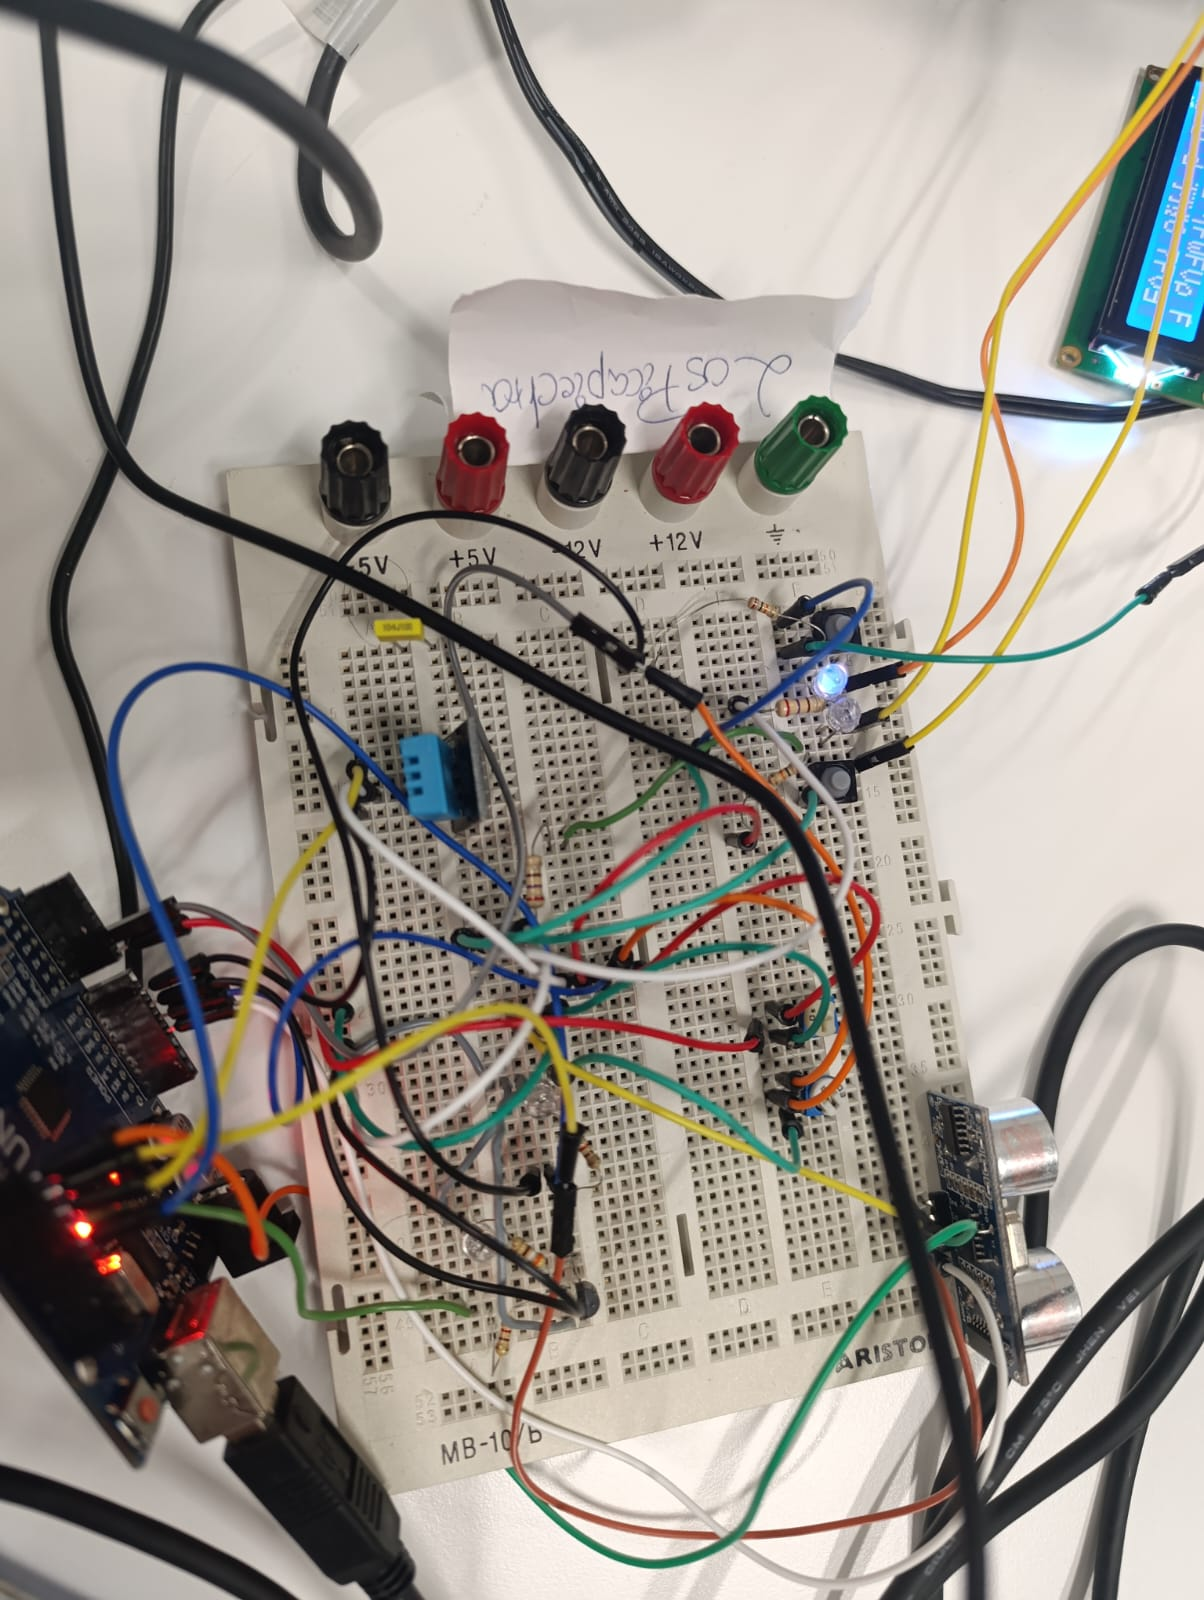
\includegraphics[width=0.7\textwidth]{imagenes/fotos-circuito/circuitocompleto1.jpeg}
        \caption*{Montaje final del sistema}
    \end{figure}

    \vfill
    \begin{tabular}{rl}
        \textbf{Autor:}      & Pablo Galilea Valverde \\[4pt]
        \textbf{Asignatura:} & Instalación y Mantenimiento de Computadores \\[4pt]
        \textbf{Titulación:} & Grado en Ingeniería Informática \\[4pt]
        \textbf{Fecha:}      & \today \\[4pt]
        \textbf{Entrega:}    & 15 de mayo de 2026 \\
    \end{tabular}
\end{titlepage}

\tableofcontents
\newpage

% ╔═══════════════════════════════════════════════════════════════════╗
% ║                      1. INTRODUCCIÓN                              ║
% ╚═══════════════════════════════════════════════════════════════════╝
\section{Introducción}

El presente documento recoge la memoria técnica del proyecto final de la asignatura
\textit{Instalación y Mantenimiento de Computadores} (Sistemas Empotrados II), consistente
en el diseño, implementación y documentación de un sistema IoT para la \textbf{automatización
y monitorización de un terrario} de pequeñas dimensiones.

El sistema permite vigilar y controlar las condiciones ambientales del terrario
(temperatura, humedad y detección de fugas) garantizando el confort de los seres
vivos que lo habitan. Para ello se integran dos plataformas hardware ---un
microcontrolador \textbf{Arduino UNO} y un minicomputador \textbf{Raspberry Pi 3B+}---
junto con la plataforma de visualización en la nube \textbf{ThingSpeak}.

\subsection{Objetivos}

\begin{itemize}[noitemsep]
    \item Diseñar e implementar un sistema de adquisición de datos con Arduino UNO
          que lea temperatura, humedad y distancia por ultrasonidos cada segundo
          mediante interrupción de \textit{timer} hardware.
    \item Controlar un ventilador y un sistema de iluminación mediante señal PWM,
          ajustables tanto manualmente (potenciómetros) como remotamente (ThingSpeak).
    \item Integrar una interfaz de usuario local con Raspberry Pi 3B+: pantalla LCD,
          botones de inicio/alarma e indicadores LED.
    \item Publicar y visualizar los datos del sistema en ThingSpeak con actualización
          cada 30 segundos.
    \item Detectar posibles fugas del animal mediante sensor de barrera de ultrasonidos
          en la puerta del terrario.
\end{itemize}

\newpage

% ╔═══════════════════════════════════════════════════════════════════╗
% ║             2. DESCRIPCIÓN GENERAL DEL SISTEMA                    ║
% ╚═══════════════════════════════════════════════════════════════════╝
\section{Descripción general del sistema}

\subsection{Arquitectura del sistema}

El sistema se compone de tres subsistemas que se comunican formando una arquitectura
en dos niveles:

\begin{enumerate}
    \item \textbf{Subsistema Arduino UNO}: nodo sensor/actuador. Adquiere datos de
          los sensores y controla los actuadores físicos del terrario.
    \item \textbf{Subsistema Raspberry Pi 3B+}: nodo de control central. Gestiona la
          comunicación serie con el Arduino, la interfaz de usuario local y la
          comunicación con la nube.
    \item \textbf{Plataforma ThingSpeak}: almacena y visualiza los datos, y permite
          el control remoto de actuadores mediante una interfaz web.
\end{enumerate}

\subsection{Diagrama de flujo general}

La figura~\ref{fig:diagrama} muestra el diagrama de flujo del sistema completo,
incluyendo la interacción entre los tres subsistemas.

% Para generar diagrama.png desde el SVG:
%   Abrir imagenes/diagrama.svg en el navegador y exportar como PNG
%   o ejecutar: inkscape --export-type=png --export-dpi=200 imagenes/diagrama.svg
\begin{figure}[H]
    \centering
    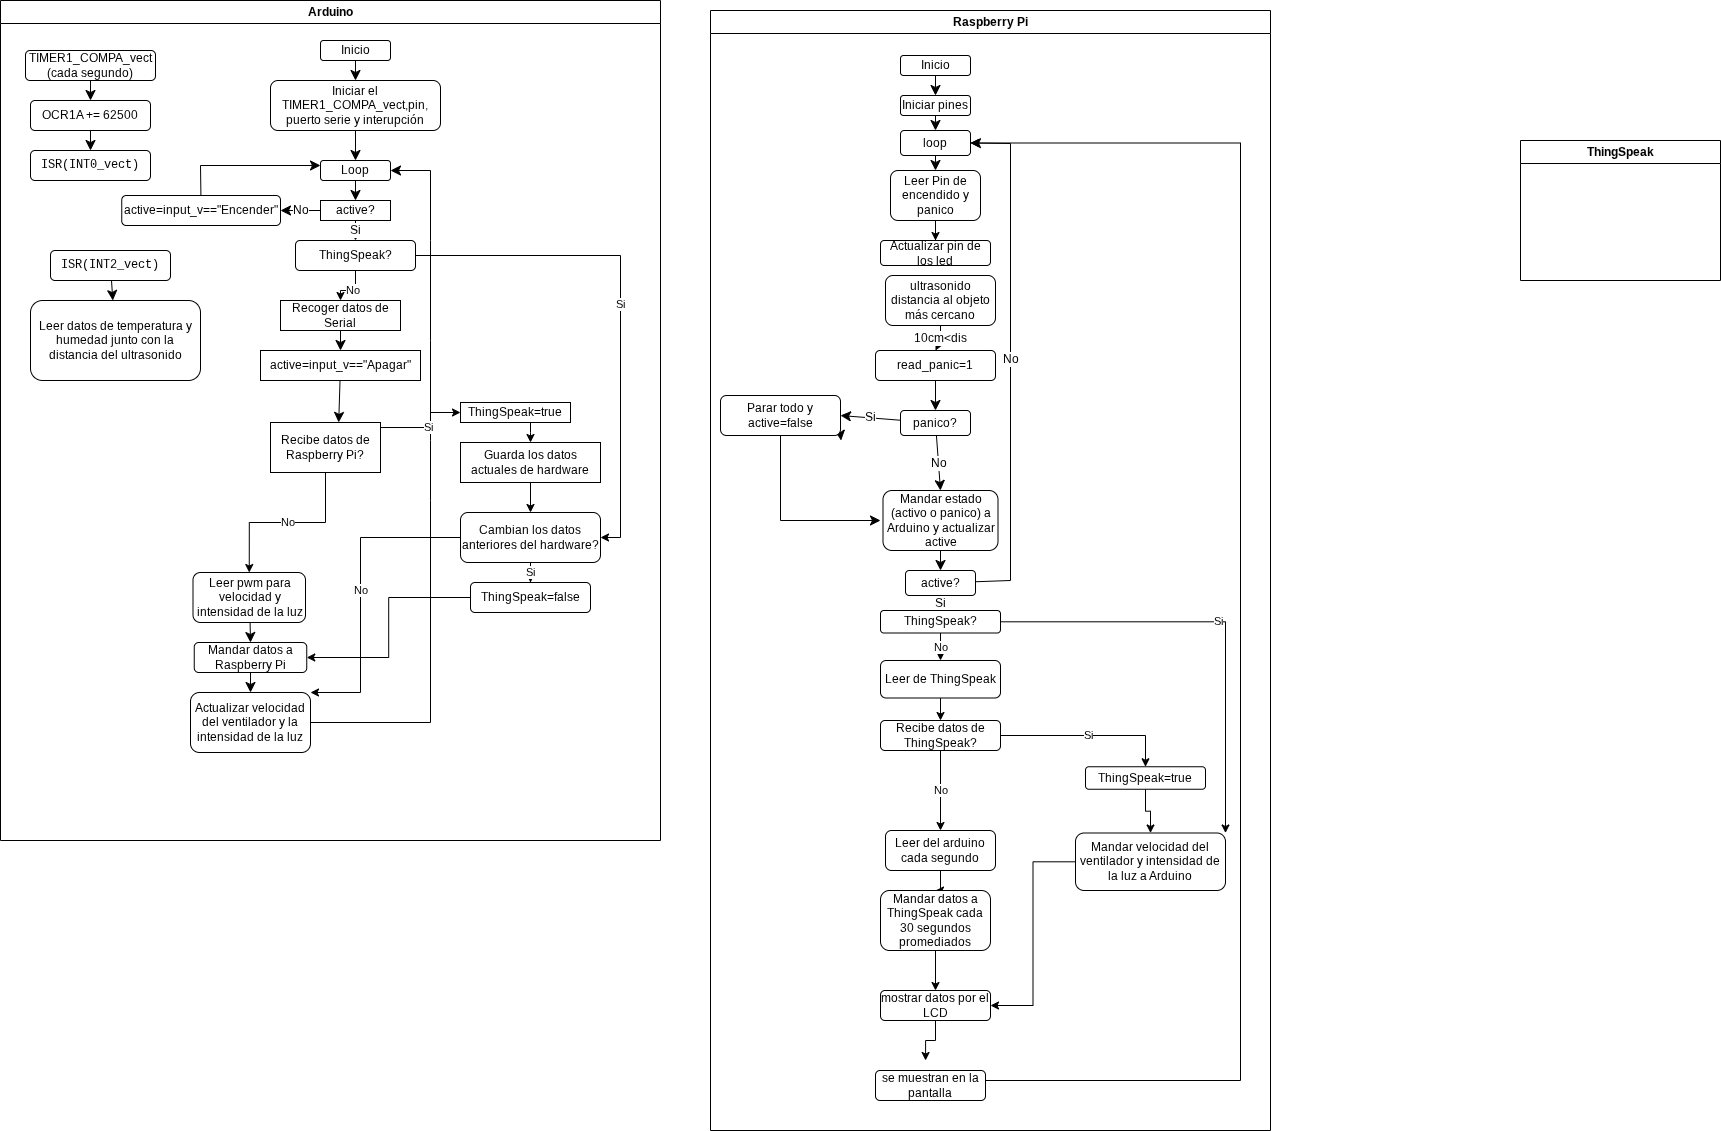
\includegraphics[width=0.95\textwidth]{imagenes/diagrama.png}
    \caption{Diagrama de flujo del sistema completo}
    \label{fig:diagrama}
\end{figure}

\subsection{Sensores y actuadores}

\begin{table}[H]
    \centering
    \caption{Sensores y actuadores del sistema}
    \label{tab:componentes}
    \renewcommand{\arraystretch}{1.3}
    \begin{tabularx}{\textwidth}{>{\bfseries}l l l X}
        \toprule
        Componente          & Tipo      & Nodo    & Función \\
        \midrule
        DHT11               & Sensor    & Arduino & Temperatura y humedad relativa \\
        HC-SR04             & Sensor    & Arduino & Distancia por ultrasonidos (detección de fuga) \\
        Potenciómetro 1     & Entrada   & Arduino & Control manual de velocidad del ventilador \\
        Potenciómetro 2     & Entrada   & Arduino & Control manual de intensidad de iluminación \\
        Ventilador (PWM)    & Actuador  & Arduino & Regulación de temperatura \\
        Tira LED (PWM)      & Actuador  & Arduino & Iluminación del terrario \\
        Botón INICIO        & Entrada   & RPi 3B+ & Arranque/parada del sistema \\
        Botón ALARMA        & Entrada   & RPi 3B+ & Activación/desactivación manual de alarma \\
        LED ESTADO          & Indicador & RPi 3B+ & Sistema activo/inactivo \\
        LED ALARMA          & Indicador & RPi 3B+ & Estado de alarma \\
        Pantalla LCD 16×2   & Salida    & RPi 3B+ & Visualización local de datos y estado \\
        \bottomrule
    \end{tabularx}
\end{table}

\subsection{Protocolo de comunicación serie}

La comunicación entre Arduino y Raspberry Pi se realiza por \textbf{UART a 9600 bps}
sobre USB (\texttt{/dev/ttyUSB0}). El Arduino envía tramas con el siguiente formato:

\begin{center}
\ttfamily V:\textit{val}\ L:\textit{val}\ T:\textit{val}\ H:\textit{val}\ D:\textit{val}\textbackslash{}n
\end{center}

donde \texttt{V} es velocidad del ventilador (0--1023), \texttt{L} intensidad de
iluminación (0--1023), \texttt{T} temperatura (\textdegree C), \texttt{H} humedad (\%)
y \texttt{D} distancia (cm). La Raspberry Pi envía comandos de control:
\texttt{encender}, \texttt{apagar}, o los valores enteros de velocidad e intensidad.

\newpage

% ╔═══════════════════════════════════════════════════════════════════╗
% ║              3. SUBSISTEMA ARDUINO UNO                            ║
% ╚═══════════════════════════════════════════════════════════════════╝
\section{Subsistema Arduino UNO}
\label{sec:arduino}

\subsection{Descripción funcional}

El Arduino UNO actúa como nodo sensor/actuador. Sus funciones son:

\begin{itemize}[noitemsep]
    \item Leer el DHT11 y el HC-SR04 cada segundo mediante interrupción de
          \textit{timer} hardware (Timer1).
    \item Leer los dos potenciómetros analógicos para el control manual de los
          actuadores.
    \item Generar señales PWM para el ventilador y la iluminación a través de
          transistores MOSFET IRL540n.
    \item Enviar los datos adquiridos a la Raspberry Pi por puerto serie y recibir
          los valores de control remoto.
    \item Gestionar la lógica de activación/desactivación del sistema.
\end{itemize}

\subsection{Esquema eléctrico}

Las figuras~\ref{fig:esquema_visual} y~\ref{fig:esquema_tecnico} muestran el esquema
eléctrico del subsistema Arduino, tanto en representación visual (Fritzing) como en
notación técnica de circuitos.

\begin{figure}[H]
    \centering
    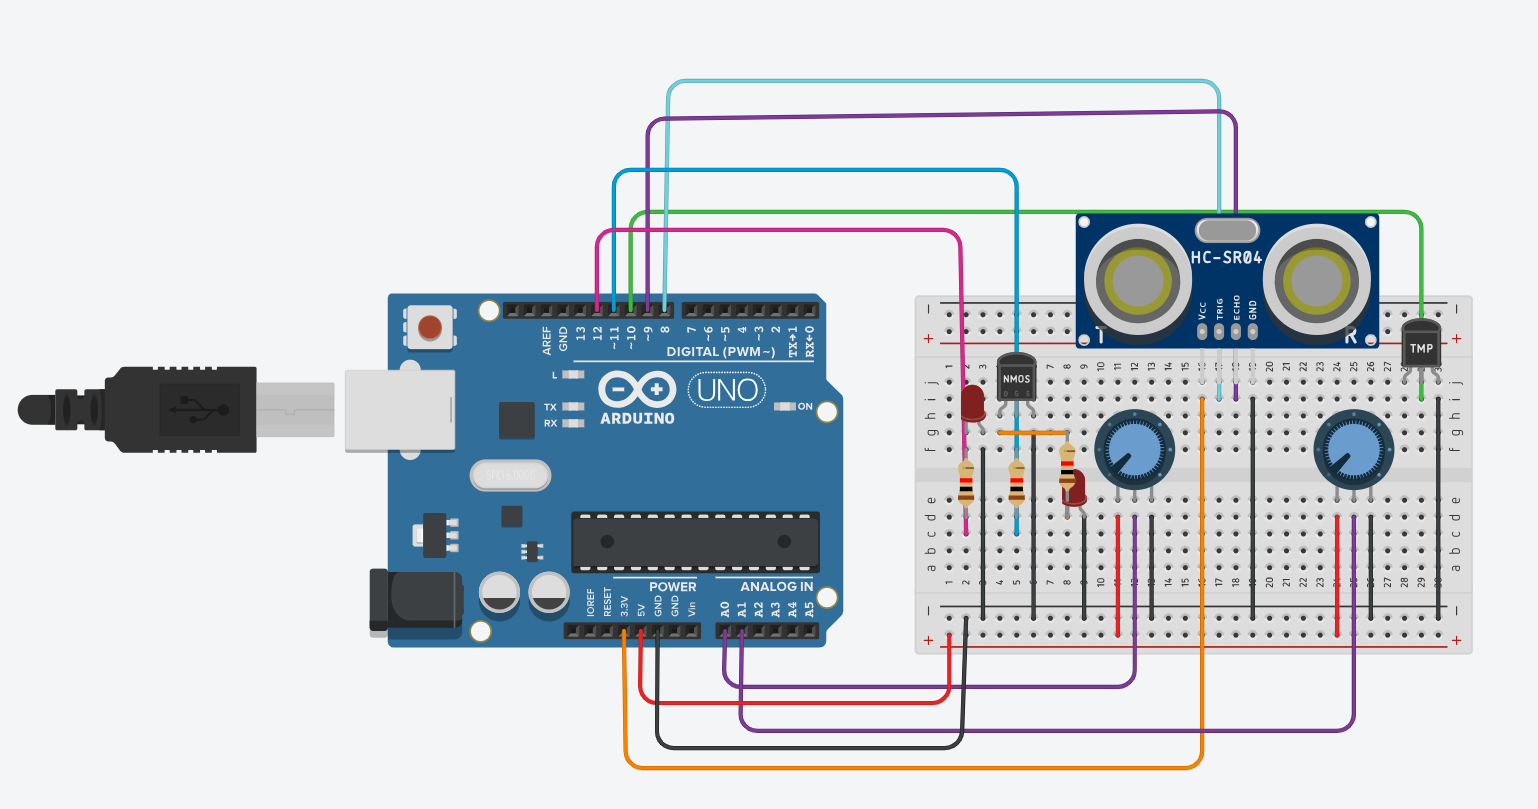
\includegraphics[width=0.92\textwidth]{imagenes/esquema-electrico/esquemaelectrico-visual.png}
    \caption{Esquema eléctrico visual del subsistema Arduino (Fritzing)}
    \label{fig:esquema_visual}
\end{figure}

\begin{figure}[H]
    \centering
    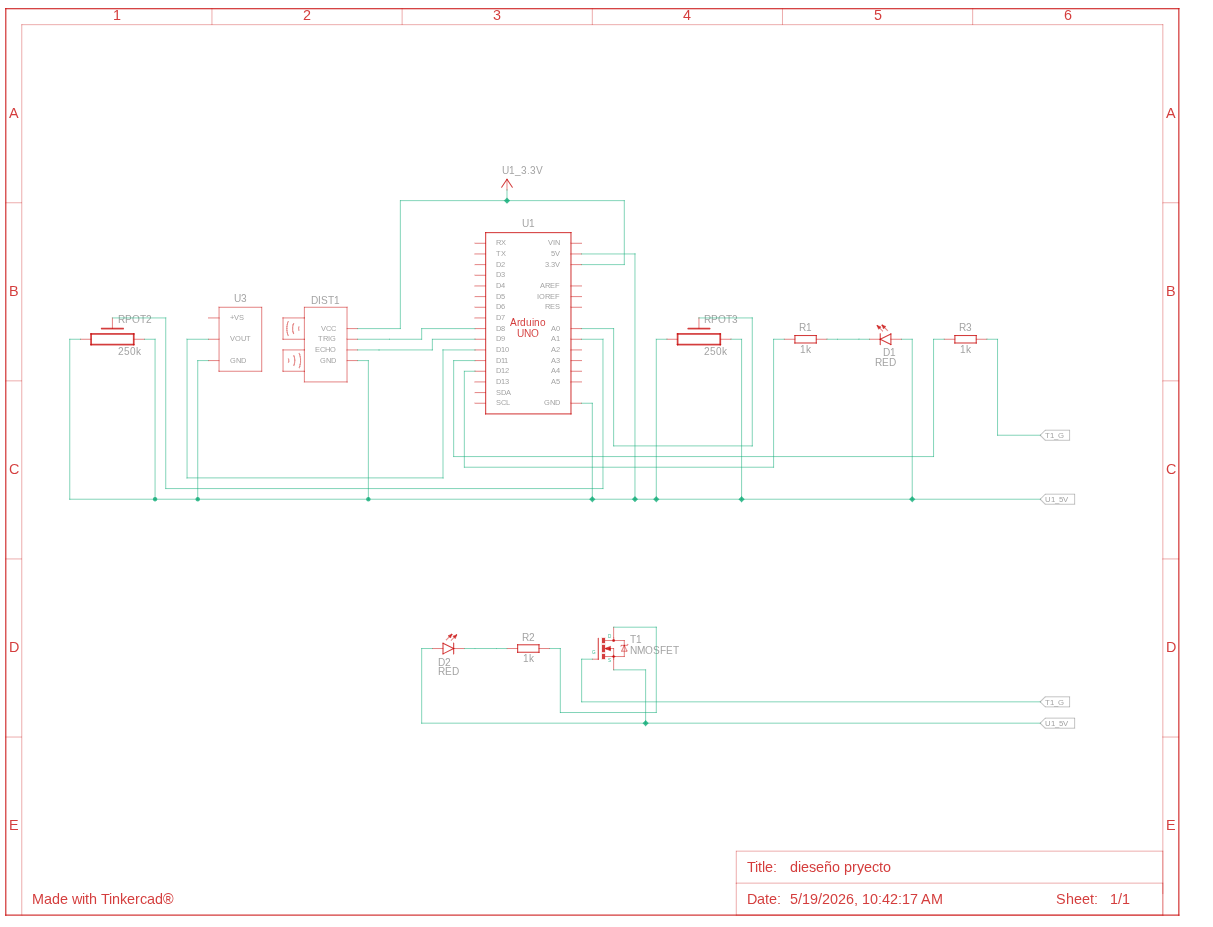
\includegraphics[width=0.92\textwidth]{imagenes/esquema-electrico/esque-electrico-serio.png}
    \caption{Esquema eléctrico técnico del subsistema Arduino}
    \label{fig:esquema_tecnico}
\end{figure}

\subsection{Descripción del circuito de potencia (MOSFET IRL540n)}

El control de los actuadores se realiza mediante transistores MOSFET de canal N
\textbf{IRL540n}. Este transistor se elige por su baja tensión umbral de puerta
($V_{GS(th)} \approx 1{,}0$\,V), compatible con los niveles lógicos de 5\,V del
Arduino, y su baja resistencia de conducción ($R_{DS(on)} < 77\,\text{m}\Omega$),
que minimiza la disipación de calor.

\begin{notatecnica}
El circuito de cada actuador incluye una \textbf{resistencia de puerta} R1
($\approx 220\,\Omega$) para limitar la corriente transitoria al cargar la
capacidad parásita de la puerta, y una \textbf{resistencia}
R2 ($\approx 10\,\text{k}\Omega$) para garantizar que el MOSFET permanece
en corte cuando el pin Arduino está en alta impedancia (por ejemplo, durante
el arranque).
\end{notatecnica}

La señal PWM del Arduino (pines 11 y 12, frecuencia $\approx 490$\,Hz) varía el ciclo
de trabajo del MOSFET, regulando la potencia media entregada al actuador de forma
proporcional al valor 0--255 escrito con \texttt{analogWrite()}.

\subsection{Interrupción del Timer1 y lectura de sensores}

\subsubsection{Configuración del Timer1}

El Arduino UNO utiliza el \textbf{Timer1} (16 bits) en modo CTC (\textit{Clear Timer
on Compare Match}) para generar una interrupción exactamente cada segundo. La
configuración se realiza directamente sobre los registros hardware:

\begin{lstlisting}[style=arduino, caption={Configuración del Timer1 en setup()}]
TCCR1A = 0;           // modo normal (no PWM)
TCCR1B = 0;
TCCR1B |= B00000100;  // prescaler = 256
OCR1A   = 62500;      // valor de comparacion
TIMSK1 |= B00000010;  // habilitar interrupcion COMPA
\end{lstlisting}

\begin{notatecnica}
Con el oscilador del Arduino UNO a 16\,MHz y un prescaler de 256, el timer avanza a:
\[
f_{tick} = \frac{16\,\text{MHz}}{256} = 62{,}500\,\text{kHz}
\]
Al fijar \texttt{OCR1A = 62500}, el timer tarda exactamente
$62500 / 62500\,\text{Hz} = \mathbf{1\,\text{s}}$ en alcanzar el valor de comparación
y lanzar la interrupción. En lugar de resetear el contador, la ISR avanza el registro
\texttt{OCR1A += 62500} sobre el contador libre, lo que garantiza que no se acumula
ningún error de tiempo entre interrupciones sucesivas.
\end{notatecnica}

\subsubsection{Rutina de servicio de interrupción (ISR)}

Cada segundo, la ISR llama a la función de lectura de sensores:

\begin{lstlisting}[style=arduino, caption={ISR del Timer1 y función de lectura}]
ISR(TIMER1_COMPA_vect)
{
  OCR1A += 62500;   // avanzar el registro para la proxima interrupcion
  INT2_vect();      // leer sensores
}

void INT2_vect() {
  humedad    = dht.readHumidity();
  temperatura = dht.readTemperature();
  if (isnan(temperatura)) { temperatura = -1; }
  if (isnan(humedad))     { humedad     = -1; }

  digitalWrite(trigger, HIGH);
  delayMicroseconds(10);
  digitalWrite(trigger, LOW);
  long duracion = pulseIn(echo, HIGH);
  // duracion en us; dividir por 59 da distancia en cm
}
\end{lstlisting}

\begin{notatecnica}
La función \texttt{INT2\_vect} se registra también como callback del pin de
interrupción por cambio de pin (\texttt{PinChangeInterrupt}), lo que permite que
el mismo código de lectura pueda invocarse tanto por el timer como por un flanco
externo. La llamada a \texttt{pulseIn()} dentro de la ISR bloquea hasta recibir
el eco del HC-SR04; a las distancias del terrario (típicamente 5--50 cm) el
tiempo de espera es inferior a 3\,ms, aceptable dentro del contexto de la ISR.

La conversión de la duración del pulso a centímetros utiliza el factor:
\[
d\,(\text{cm}) = \frac{t\,(\mu\text{s})}{58{,}82} \approx \frac{t}{59}
\]
derivado de la velocidad del sonido ($v \approx 343$\,m/s) y el trayecto de ida
y vuelta del pulso ($d = v \cdot t / 2$).
\end{notatecnica}

\subsection{Lógica de control y protocolo de prioridad}

El Arduino implementa una máquina de estados simple con dos variables booleanas:
\texttt{active} (sistema encendido) y \texttt{ThingSpeak} (control remoto activo).

\begin{notatecnica}
La variable \texttt{ThingSpeak} actúa como \textbf{indicador de prioridad} entre
el control manual y el remoto. Cuando la Raspberry Pi envía un comando de velocidad
o intensidad, \texttt{ThingSpeak} se pone a \texttt{true} y el Arduino ignora los
potenciómetros hasta que detecta un cambio en ellos, momento en que devuelve la
prioridad al control local (\texttt{ThingSpeak = false}). Esto evita conflictos
cuando el usuario gira un potenciómetro mientras hay un comando remoto activo.
\end{notatecnica}

\newpage

% ╔═══════════════════════════════════════════════════════════════════╗
% ║            4. SUBSISTEMA RASPBERRY PI 3B+                         ║
% ╚═══════════════════════════════════════════════════════════════════╝
\section{Subsistema Raspberry Pi 3B+}

\subsection{Descripción funcional}

La Raspberry Pi 3B+ actúa como nodo de control central. Sus funciones son:

\begin{itemize}[noitemsep]
    \item Leer los datos del Arduino por puerto serie cada segundo.
    \item Mostrar temperatura, humedad y estado en la pantalla LCD 16×2.
    \item Gestionar los botones físicos de inicio y alarma.
    \item Controlar los LEDs indicadores de estado.
    \item Publicar datos promediados en ThingSpeak cada 30 segundos.
    \item Recibir comandos de control de ThingSpeak y reenviarlos al Arduino.
    \item Activar la alarma automáticamente si la distancia es inferior a 10\,cm.
\end{itemize}

\subsection{Fotografías del montaje}

\begin{figure}[H]
    \centering
    \begin{subfigure}[b]{0.48\textwidth}
        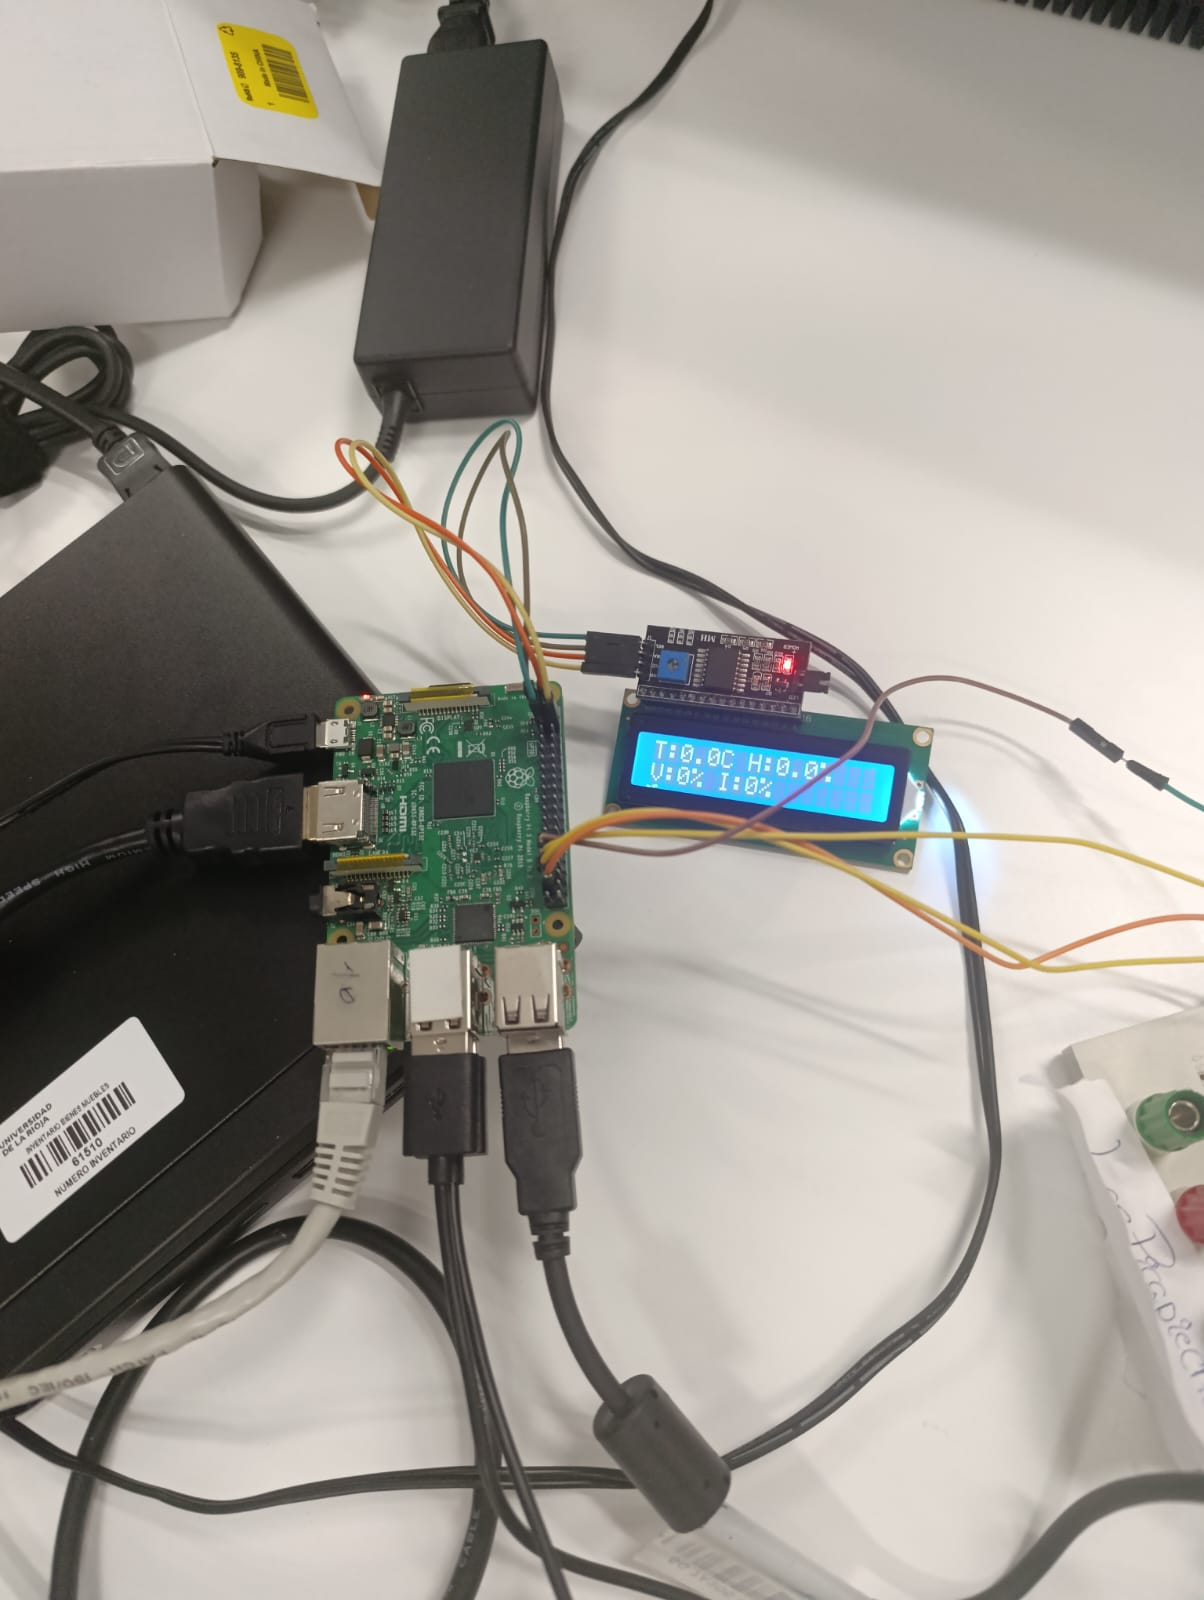
\includegraphics[width=\textwidth]{imagenes/fotos-circuito/arduino-pantalla-bien.jpeg}
        \caption{Arduino y pantalla LCD funcionando correctamente}
    \end{subfigure}
    \hfill
    \begin{subfigure}[b]{0.48\textwidth}
        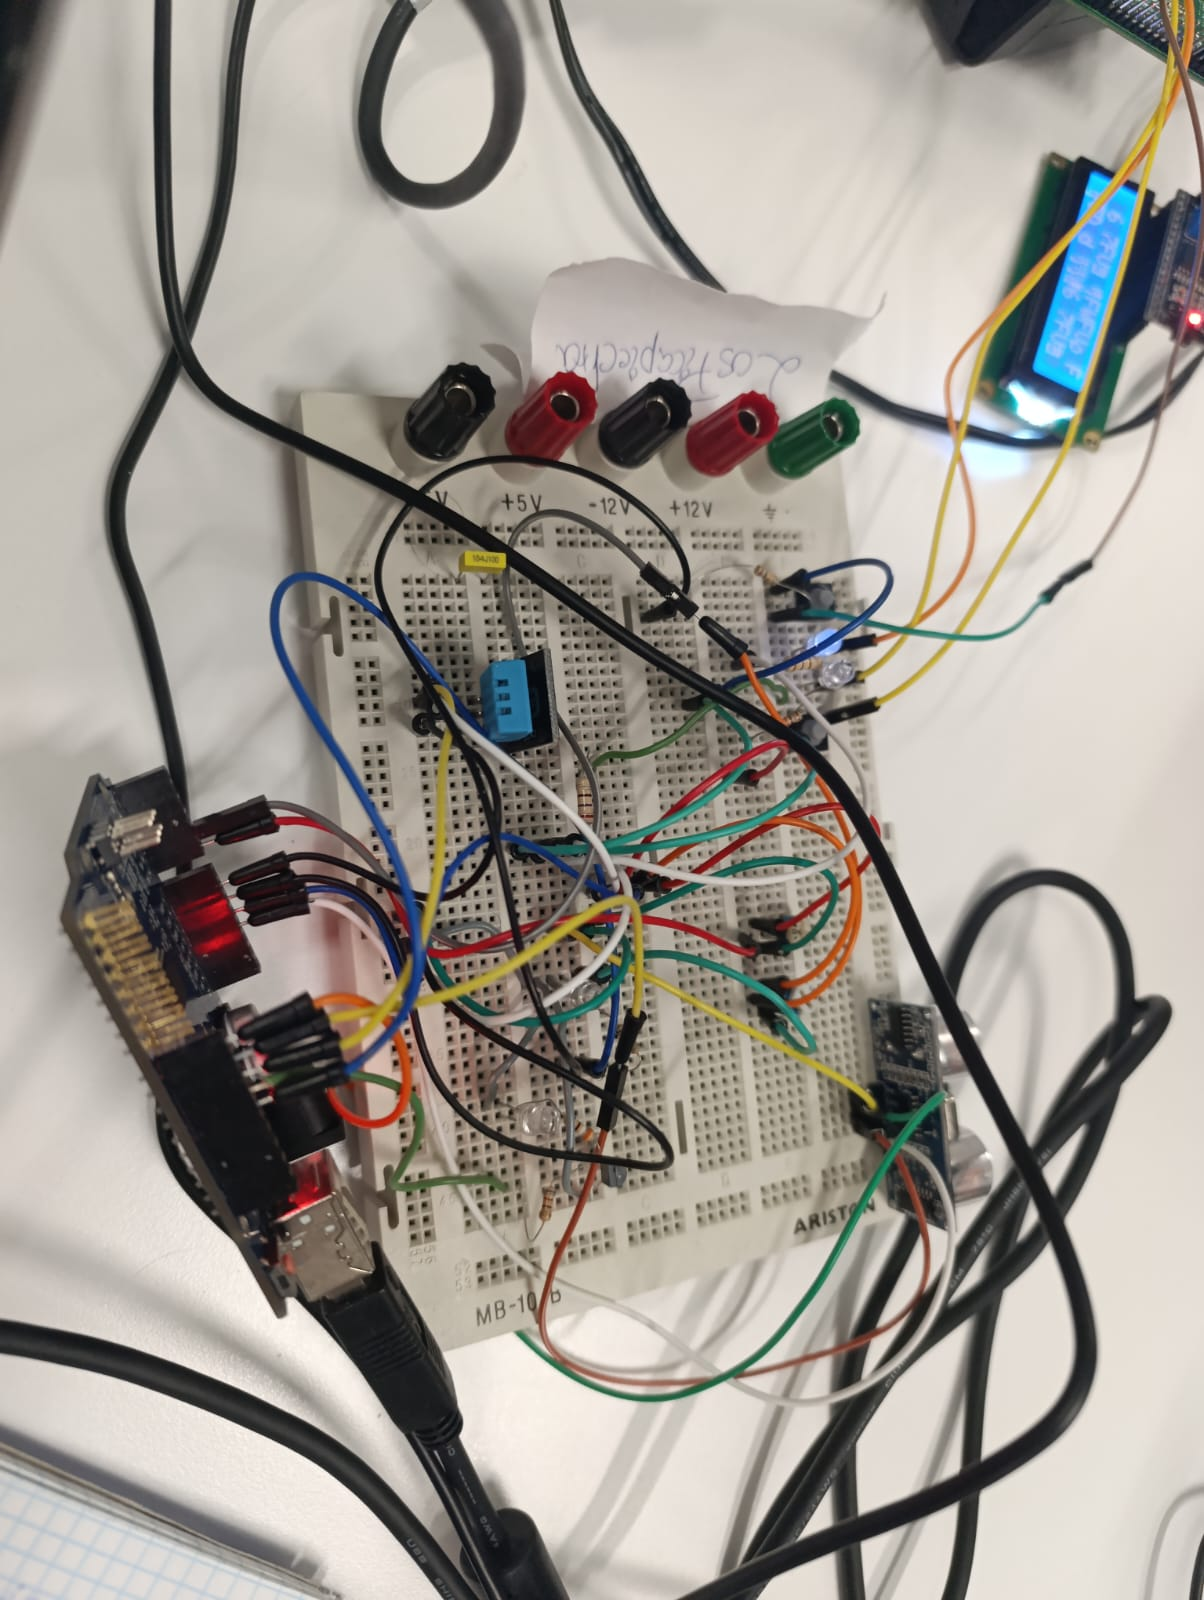
\includegraphics[width=\textwidth]{imagenes/fotos-circuito/cablescircuito.jpeg}
        \caption{Detalle del cableado del circuito}
    \end{subfigure}
    \caption{Fotografías del montaje hardware}
    \label{fig:montaje}
\end{figure}

\begin{figure}[H]
    \centering
    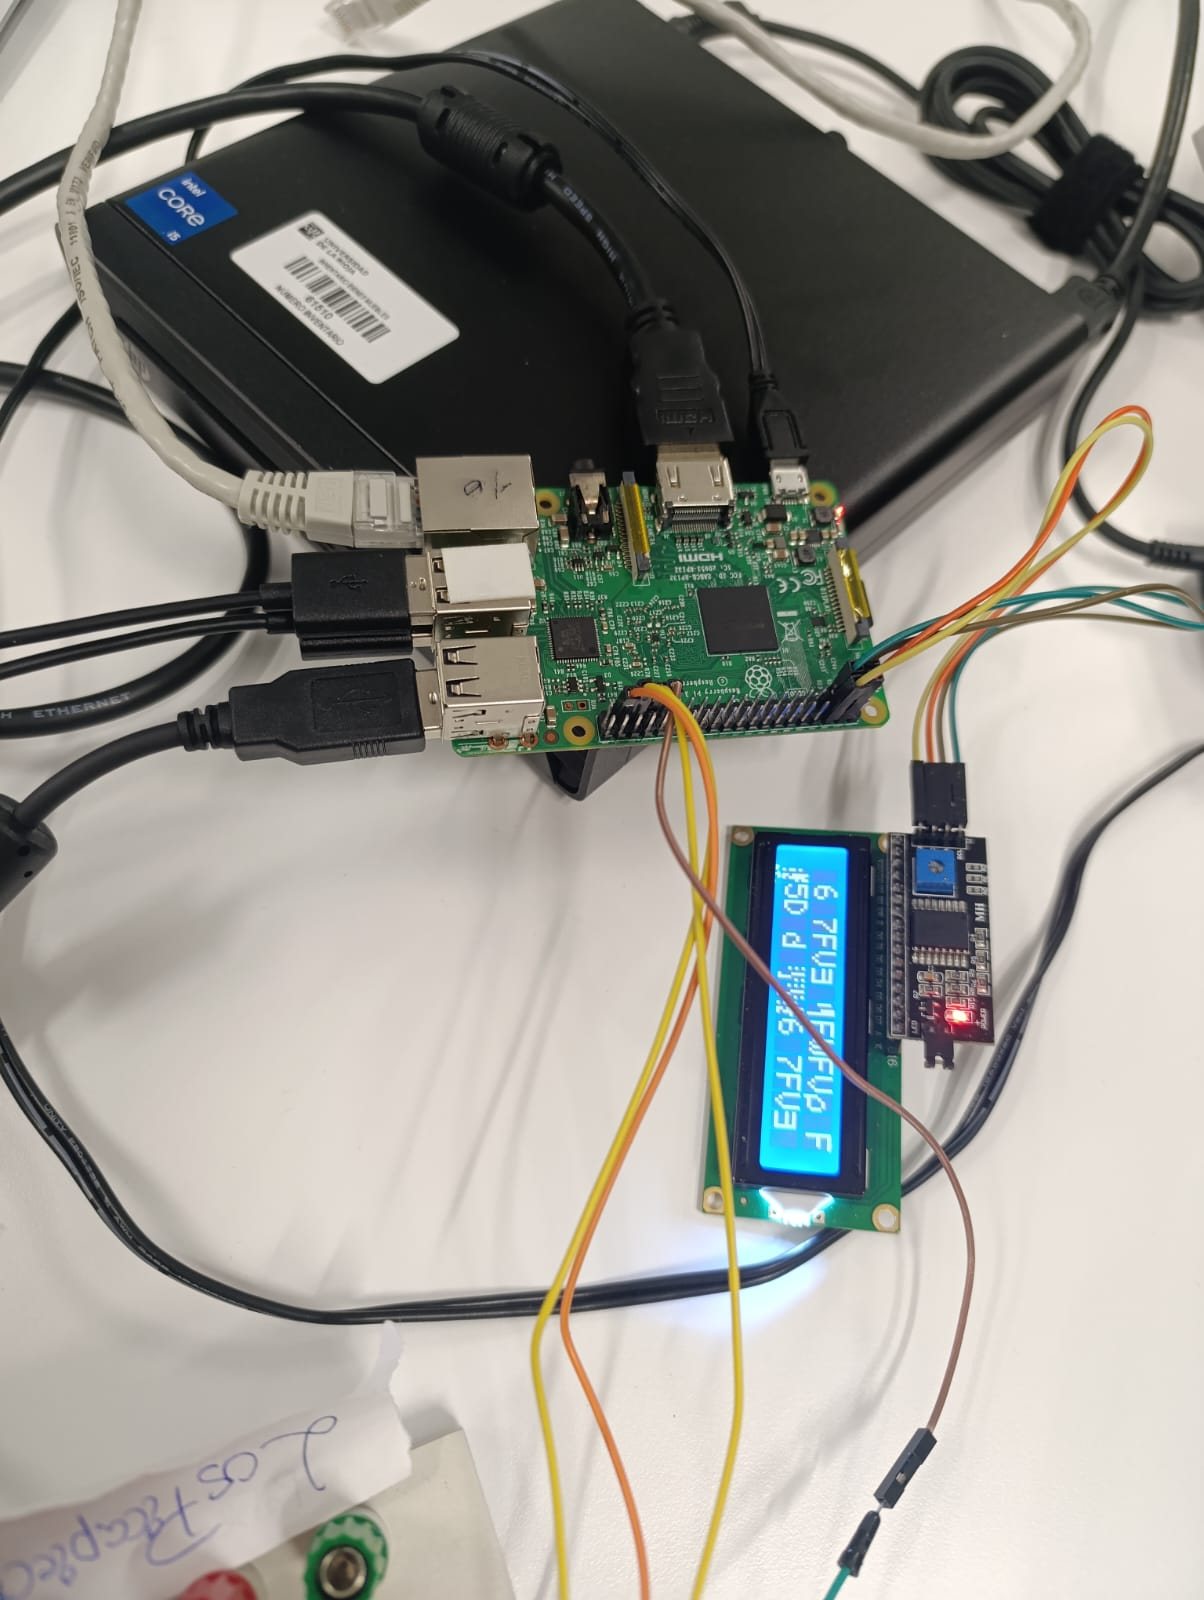
\includegraphics[width=0.7\textwidth]{imagenes/fotos-circuito/arduinoypantalla-pantallamal.jpeg}
    \caption{Prueba de la pantalla LCD durante el proceso de depuración}
    \label{fig:pantalla_debug}
\end{figure}

\subsection{Modelo de hilos (\textit{threading})}

El programa Python utiliza \textbf{tres hilos de ejecución} para gestionar las tareas
concurrentes sin bloquear el bucle principal:

\begin{itemize}[noitemsep]
    \item \textbf{Hilo principal}: lee datos serie del Arduino e invoca
          \texttt{update\_lcd()} continuamente.
    \item \textbf{Hilo ThingSpeak} (\texttt{thingspeak\_thread}): envía datos
          promediados y lee comandos cada 30 segundos.
    \item \textbf{Hilo de botones} (\texttt{button\_thread}): sondea los pines GPIO
          con anti-rebote por software.
\end{itemize}

\begin{notatecnica}
Los tres hilos acceden a las variables globales \texttt{active}, \texttt{alarm},
\texttt{ventilador\_cmd} e \texttt{iluminacion\_cmd} sin mutex explícito. Esto es
seguro en CPython gracias al \textbf{GIL} (\textit{Global Interpreter Lock}), que
garantiza que solo un hilo ejecuta bytecode Python en cada instante. En un intérprete
sin GIL (como PyPy o CPython 3.13+ sin GIL) sería necesario usar \texttt{threading.Lock}.
\end{notatecnica}

\subsubsection{Anti-rebote por software en el hilo de botones}

El hilo de botones implementa detección de \textbf{flanco de subida} por software:

\begin{lstlisting}[style=python, caption={Detección de flanco en button\_thread}]
last_encender = False
while True:
    encender = GPIO.input(BOTON_ENCENDER)
    if encender and not last_encender:   # flanco de subida
        active = not active
        send_command_to_arduino("encender" if active else "apagar")
        update_leds()
        update_lcd()
    last_encender = encender
\end{lstlisting}

\begin{notatecnica}
La comparación \texttt{encender and not last\_encender} detecta el flanco ascendente
(transición \texttt{False}$\to$\texttt{True}) sin necesidad de \texttt{sleep()} ni
\texttt{GPIO.add\_event\_detect()}. Esta técnica, conocida como
\textit{edge detection by polling}, es robusta frente al rebote mecánico del
pulsador siempre que el bucle tarde más que el tiempo de rebote típico ($\sim$5 ms),
lo que se cumple dado que el hilo realiza operaciones serie y de red.
\end{notatecnica}

\subsection{Buffer de datos y promediado para ThingSpeak}

Los datos recibidos del Arduino se almacenan en una \texttt{deque} de tamaño máximo
300 muestras. Cada vez que el hilo ThingSpeak se activa (cada 30 s), calcula el
promedio de todas las muestras acumuladas y las envía a la nube:

\begin{lstlisting}[style=python, caption={Cálculo de promedios en send\_to\_thingspeak()}]
data_buffer = deque(maxlen=300)   # hasta ~5 min de muestras a 1 Hz

# En send_to_thingspeak():
temps  = [d[2] for d in data_buffer]
avg_temp = sum(temps) / len(temps)
# ... igualmente para humedad, distancia, velocidad, intensidad
\end{lstlisting}

\begin{notatecnica}
Al usar \texttt{deque(maxlen=300)}, el buffer descarta automáticamente las muestras
más antiguas cuando se supera la capacidad. Esto significa que si la RPi no consigue
enviar a ThingSpeak durante varios intervalos de 30 s (por ejemplo, por pérdida de
conexión Wi-Fi), el promedio enviado al recuperar la conexión refleja hasta los
últimos 5 minutos de datos en lugar de solo los últimos 30 segundos. Las muestras
anteriores al fallo se pierden, pero el sistema no colapsa ni acumula memoria de
forma indefinida.
\end{notatecnica}

\subsection{Detección automática de alarma}

Dentro de \texttt{read\_serial\_data()}, cada muestra de distancia se comprueba
contra el umbral de 10\,cm:

\begin{lstlisting}[style=python, caption={Detección automática de fuga}]
if dist > 0 and dist < 10 and not alarm:
    alarm = True
    update_leds()
    send_command_to_arduino("apagar")
    lcd.clear()
    lcd.message("ALARMA! Fuga", 1)
    lcd.message("Dist < 10 cm", 2)
\end{lstlisting}

La condición \texttt{dist > 0} filtra las lecturas erróneas del HC-SR04 (valor 0
cuando no hay eco). La alarma solo se activa una vez (\texttt{not alarm}) y debe
desactivarse manualmente mediante el botón de pánico.

\newpage

% ╔═══════════════════════════════════════════════════════════════════╗
% ║             5. INTERFAZ EN LA NUBE: THINGSPEAK                    ║
% ╚═══════════════════════════════════════════════════════════════════╝
\section{Interfaz en la nube: ThingSpeak}
\label{sec:thingspeak}

\subsection{Configuración del canal}

Se configura un canal ThingSpeak con ocho campos según la tabla~\ref{tab:thingspeak}.
Los datos de lectura (fields 1--4) se publican como promedios de los últimos 30
segundos; los campos de control (fields 5--6) son escritos por el usuario desde la
interfaz web y leídos por la RPi.

\begin{table}[H]
    \centering
    \caption{Configuración de campos en ThingSpeak}
    \label{tab:thingspeak}
    \renewcommand{\arraystretch}{1.3}
    \begin{tabular}{cllc}
        \toprule
        \textbf{Field} & \textbf{Nombre}              & \textbf{Descripción}                & \textbf{Dirección} \\
        \midrule
        1 & Temperatura (\textdegree C)              & Promedio 30 s (DHT11)               & RPi $\to$ TS \\
        2 & Humedad (\%)                             & Promedio 30 s (DHT11)               & RPi $\to$ TS \\
        3 & Distancia (cm)                           & Promedio 30 s (HC-SR04)             & RPi $\to$ TS \\
        4 & Estado alarma                            & 0 = normal, 1 = alarma              & RPi $\to$ TS \\
        5 & Velocidad ventilador (\%)                & Comando usuario (0--100)            & TS $\to$ RPi \\
        6 & Intensidad iluminación (\%)              & Comando usuario (0--100)            & TS $\to$ RPi \\
        7 & Velocidad real ventilador                & Valor ADC potenciómetro (0--1023)   & RPi $\to$ TS \\
        8 & Intensidad real iluminación              & Valor ADC potenciómetro (0--1023)   & RPi $\to$ TS \\
        \bottomrule
    \end{tabular}
\end{table}

\subsection{Comunicación REST con ThingSpeak}

La RPi realiza las peticiones HTTP directamente con \texttt{urllib.request} sin
dependencias externas. La escritura se realiza mediante una petición GET con los
parámetros en la URL:

\begin{lstlisting}[style=python, caption={Escritura en ThingSpeak (send\_to\_thingspeak)}]
url  = f"https://api.thingspeak.com/update?api_key={WRITE_API_KEY}"
url += f"&field1={avg_temp}&field2={avg_hum}&field3={avg_dist}"
url += f"&field4={1 if alarm else 0}"
url += f"&field5={ventilador_cmd}&field6={iluminacion_cmd}"
url += f"&field7={avg_vel}&field8={avg_lum}"
urllib.request.urlopen(url, timeout=5)
\end{lstlisting}

La lectura de comandos recupera el último \textit{feed} del canal y extrae los campos 5 y 6:

\begin{lstlisting}[style=python, caption={Lectura de comandos desde ThingSpeak}]
url = f"https://api.thingspeak.com/channels/{CHANNEL_ID}/feeds.json" \
      f"?api_key={READ_API_KEY}"
response = urllib.request.urlopen(url, timeout=5)
data = json.loads(response.read().decode())
new_vent = int(float(data['field5']))
\end{lstlisting}

\begin{notatecnica}
Ambas peticiones incluyen \texttt{timeout=5} para evitar que un fallo de red bloquee
el hilo ThingSpeak indefinidamente. Los errores se capturan con
\texttt{urllib.error.URLError} y se imprimen por consola, pero no interrumpen la
ejecución, lo que garantiza la continuidad del sistema aunque la conexión a internet
sea intermitente.
\end{notatecnica}

\subsection{Resultados obtenidos en ThingSpeak}

Las figuras~\ref{fig:thingspeak1} y~\ref{fig:thingspeak2} muestran las capturas
reales del canal ThingSpeak durante el funcionamiento del sistema.

\begin{figure}[H]
    \centering
    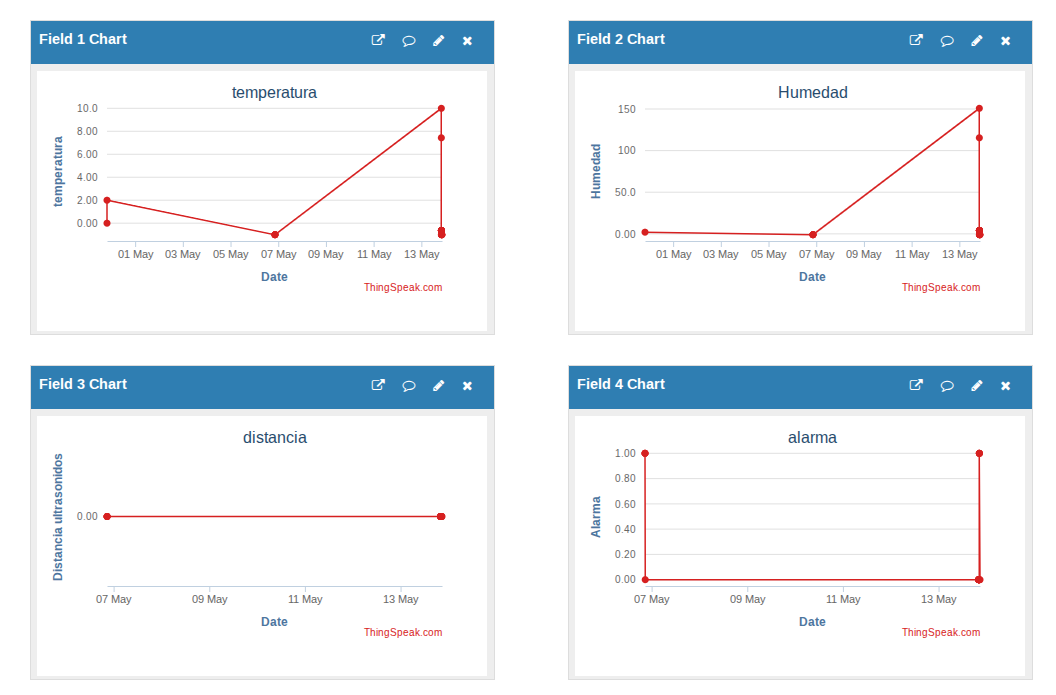
\includegraphics[width=\textwidth]{imagenes/thinkspeak/tablasthinkspeak1.png}
    \caption{Canal ThingSpeak: gráficas de temperatura, humedad y distancia}
    \label{fig:thingspeak1}
\end{figure}

\begin{figure}[H]
    \centering
    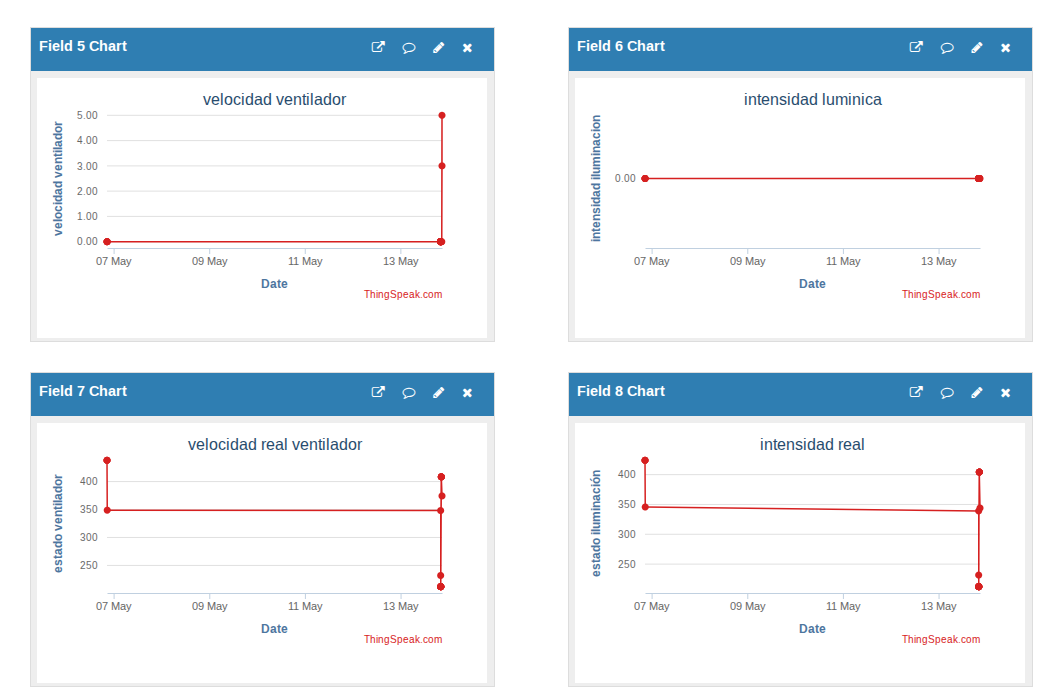
\includegraphics[width=\textwidth]{imagenes/thinkspeak/tablasthinkspeak2.png}
    \caption{Canal ThingSpeak: estado de actuadores y alarma}
    \label{fig:thingspeak2}
\end{figure}

Los resultados mostrados reflejan el comportamiento real del sistema con el hardware
disponible. Algunas lecturas presentan anomalías ---como valores de temperatura o
humedad fuera de rango o distancias inconsistentes--- atribuibles al \textbf{mal
estado de los componentes hardware} \footnote{Con mal estado me refiero a que es probable que por un cortocircuito durante el montaje, nos los cargasemos nosotros, no tiene la culpa el profesorado ni la asignatura.} utilizados: el sensor DHT11 presentó lecturas
inestables y el HC-SR04 mostró ecos espurios en determinadas condiciones.

Cabe señalar que, dado que los datos se envían mediante una simple petición HTTP
con la API key en la URL, hubiera sido trivial manipular o fabricar las medidas para
presentar un resultado más favorable. Sin embargo, se ha optado conscientemente por
\textbf{mostrar los datos reales} obtenidos durante las pruebas, ya que la honestidad
en la presentación de resultados es parte esencial del rigor de cualquier trabajo de
ingeniería. Las limitaciones observadas son una consecuencia del hardware y no del
diseño software del sistema, que funciona correctamente dentro de las restricciones
impuestas por los componentes.

\newpage

% ╔═══════════════════════════════════════════════════════════════════╗
% ║                   6. PRESUPUESTO ESTIMADO                         ║
% ╚═══════════════════════════════════════════════════════════════════╝
\section{Presupuesto estimado}

\begin{table}[H]
    \centering
    \caption{Presupuesto estimado de componentes hardware}
    \label{tab:presupuesto}
    \renewcommand{\arraystretch}{1.3}
    \begin{tabularx}{\textwidth}{X c r r}
        \toprule
        \textbf{Componente}           & \textbf{Ud.} & \textbf{P.\ unit.} & \textbf{Total} \\
        \midrule
        Arduino UNO R3                & 1  & 22,00\,€  & 22,00\,€ \\
        Raspberry Pi 3B+              & 1  & 45,00\,€  & 45,00\,€ \\
        Tarjeta microSD 16 GB         & 1  &  6,00\,€  &  6,00\,€ \\
        Sensor DHT11                  & 1  &  2,50\,€  &  2,50\,€ \\
        Sensor ultrasonidos HC-SR04   & 1  &  2,00\,€  &  2,00\,€ \\
        Transistor MOSFET IRL540n     & 2  &  0,80\,€  &  1,60\,€ \\
        Potenciómetro 10\,k$\Omega$   & 2  &  0,40\,€  &  0,80\,€ \\
        Ventilador 5\,V               & 1  &  3,50\,€  &  3,50\,€ \\
        Tira LED                      & 1  &  4,00\,€  &  4,00\,€ \\
        Pantalla LCD 16×2 con I2C     & 1  &  5,00\,€  &  5,00\,€ \\
        Pulsadores                    & 2  &  0,30\,€  &  0,60\,€ \\
        LEDs indicadores              & 2  &  0,10\,€  &  0,20\,€ \\
        Resistencias (surtido)        & 1  &  1,50\,€  &  1,50\,€ \\
        Cables y protoboard           & 1  &  5,00\,€  &  5,00\,€ \\
        \midrule
        \multicolumn{3}{r}{\textbf{TOTAL estimado}} & \textbf{100,20\,€} \\
        \bottomrule
    \end{tabularx}
\end{table}

\noindent Los precios son orientativos y pueden variar según el proveedor. No se
incluyen costes de mano de obra ni herramientas ni el factor de que es muy probable que en el proceso Pedro o Pablo rompiesen un componente hardware y se tuvise que tener material de repuesto. 

\newpage

% ╔═══════════════════════════════════════════════════════════════════╗
% ║                      7. CONCLUSIONES                              ║
% ╚═══════════════════════════════════════════════════════════════════╝
\section{Conclusiones}

\subsection{Conclusiones técnicas}

\begin{itemize}
    \item El uso de la \textbf{interrupción de Timer1} en Arduino garantiza la
          periodicidad exacta de 1 segundo en la adquisición de datos,
          independientemente de la carga del bucle principal.

    \item El control \textbf{PWM mediante MOSFET IRL540n} ofrece una solución
          eficiente y de bajo coste para la regulación de potencia en los actuadores,
          con baja disipación de calor en el transistor.

    \item La arquitectura \textbf{Arduino + Raspberry Pi} permite separar la lógica
          de control en tiempo real (Arduino) de la gestión de alto nivel y
          comunicaciones (RPi), mejorando la modularidad y mantenibilidad del sistema.

    \item El modelo de \textbf{tres hilos} en Python (principal, ThingSpeak, botones)
          permite gestionar eficientemente las tareas concurrentes sin necesidad de
          un sistema operativo en tiempo real.

    \item La plataforma \textbf{ThingSpeak} facilita la integración IoT con
          almacenamiento y visualización de datos sin infraestructura propia.
\end{itemize}

\subsection{Dificultades encontradas}

\begin{itemize}
      \item La llamada a \texttt{pulseIn()} dentro de la ISR del timer es técnicamente
          una operación bloqueante en contexto de interrupción. A las distancias
          del terrario el impacto es mínimo, pero en un diseño de producción se
          debería medir el eco mediante interrupción externa para no bloquear otras
          ISRs.

      \item La sincronización del protocolo serie entre Arduino y RPi requirió un
          cuidadoso diseño del formato de trama y el vaciado del buffer inicial al
          arrancar (\texttt{reset\_input\_buffer()}) para evitar lecturas corruptas.
      \item No se pudo comprobar el correcto funcionamiento del circuito en su totalidad porque es muy probable que quemasemos el controlador de movimiento y eso impidio que se pudiese comprobar su correcto funcionamiento.
      \item Al estar acostumbrados a manejar más software que hardware se nos ha complicado el tener que tener cuidado con el material y el no dañar nuestra integridad fisica en el proceso.
\end{itemize}



\newpage

% ╔═══════════════════════════════════════════════════════════════════╗
% ║                      8. REFERENCIAS                               ║
% ╚═══════════════════════════════════════════════════════════════════╝
\section{Referencias}

\begin{enumerate}
    \item Arduino. \textit{Arduino UNO Reference}.
          \url{https://docs.arduino.cc/hardware/uno-rev3/}
    \item Arduino. \textit{Timer1 / TCCR1 Register Description}. ATmega328P Datasheet,
          Microchip Technology.
    \item Raspberry Pi Foundation. \textit{Raspberry Pi 3B+ documentation}.
          \url{https://www.raspberrypi.com/documentation/}
    \item Aosong Electronics. \textit{DHT11 Humidity \& Temperature Sensor Datasheet}.
    \item SparkFun. \textit{HC-SR04 Ultrasonic Distance Sensor Datasheet}.
    \item International Rectifier. \textit{IRL540n HEXFET Power MOSFET Datasheet}.
    \item MathWorks. \textit{ThingSpeak Documentation}.
          \url{https://www.mathworks.com/help/thingspeak/}
    \item Python Software Foundation. \textit{threading — Thread-based parallelism}.
          \url{https://docs.python.org/3/library/threading.html}
    \item RPi.GPIO. \textit{RPi.GPIO Python Library}.
          \url{https://sourceforge.net/projects/raspberry-gpio-python/}
    \item Galilea Valverde, P. \textit{Repositorio del proyecto: Sistema IoT para
          control y monitorización de un terrario}. GitHub, 2026.
          \url{https://github.com/pagaliv/proyect-final-computadores-III}
\end{enumerate}

\newpage

% ╔═══════════════════════════════════════════════════════════════════╗
% ║                    REPRODUCIBILIDAD                               ║
% ╚═══════════════════════════════════════════════════════════════════╝
\section*{Reproducibilidad del proyecto}
\addcontentsline{toc}{section}{Reproducibilidad del proyecto}

Todo el material necesario para replicar este proyecto ---código fuente, esquemas
eléctricos, diagrama de flujo e imágenes--- está disponible públicamente en el
siguiente repositorio de GitHub:

\begin{center}
    \url{https://github.com/pagaliv/proyect-final-computadores-III}
\end{center}

La estructura del repositorio es la siguiente:

\begin{itemize}[noitemsep]
    \item \texttt{codigo/arduino/} --- Firmware del Arduino UNO (\texttt{terrario.ino})
    \item \texttt{codigo/rpi/} --- Programa de la Raspberry Pi (\texttt{cucu.py})
    \item \texttt{imagenes/} --- Esquemas eléctricos, diagrama de flujo y fotografías
          del montaje
    \item \texttt{documentacion/} --- Enunciado original de la práctica
    \item \texttt{memoria.tex} --- Fuente \LaTeX{} de este documento
\end{itemize}

Para reproducir el sistema son necesarios los componentes listados en la
sección~\ref{tab:presupuesto} y seguir los pasos descritos en las
secciones~\ref{sec:arduino} a~\ref{sec:thingspeak} de esta memoria.

\newpage

% ╔═══════════════════════════════════════════════════════════════════╗
% ║                       ANEXOS                                      ║
% ╚═══════════════════════════════════════════════════════════════════╝
\appendix
\titleformat{\section}{\large\bfseries}{Anexo \Alph{section}.}{0.5em}{}[\titlerule]

\section{Código fuente Arduino (terrario.ino)}
\label{anx:arduino}

\lstinputlisting[
    style=arduino,
    caption={Programa completo Arduino -- terrario.ino},
    label={lst:arduino}
]{codigo/arduino/terrario.ino}

\newpage

\section{Código fuente Raspberry Pi (cucu.py)}
\label{anx:python}

\lstinputlisting[
    style=python,
    caption={Programa completo Raspberry Pi -- cucu.py},
    label={lst:python}
]{codigo/rpi/cucu.py}

\end{document}
